
\chapter{Solução Proposta}
\label{cap:solucao}

Considerando os requisitos de coreografias de serviços web, de uso da computação em nuvem e de sistemas em grande escala, definimos um arcabouço para a implantação de coreografias de serviços web denominado \ee. Os serviços oferecidos pelo nosso arcabouço se integram ao Ambiente Integrado de Desenvolvimento e Execução CHOReOS, que visa fornecer todo o processo de desenvolvimento, implantação e governança de coreografias de serviços web. Para a implementação do arcabouço Enactment Engine contribuíram diretamente os seguintes colegas do grupo de pesquisa: Daniel Cuckier, Carlos Eduardo do Santos, Felipe Pontes, Alfonso Diaz, Nelson Lago e Paulo Moura. \gerosa{Será que precisa dizer? Não poderia estar nos agradecimentos?}. O código-fonte do \ee, que é software livre sob a licença LGPL\footnote{\Leo{por o link pra LGPL}}, está disponível em \url{http://www.github.com/choreos/enactment\_engine}.

Neste capítulo descrevemos a arquitetura do arcabouço proposto, incluindo os pontos de extensão previstos. Destacamos os aspectos cobertos e não cobertos dos requisitos de sistemas de grande escala. Apresentamos também o estado atual da implementação do arcabouço, assim como os resultados experimentais sobre sua escalabilidade obtidos até o momento.

\section{Arquitetura}
\label{sec:arquitetura}

As funcionalidades do Enactment Engine são expostas como serviços, sendo a principal operação disponível a encenação de coreografias. Para executar essa operação, o Enactment Engine recebe uma descrição arquitetural de baixo nível da coreografia, que contém as URLs para seus artefatos implantáveis. Com base nessa descrição, o Enactment Engine implanta os artefatos em diversos nós nas nuvens das diferentes organizações participantes da coreografia. O cliente do Enactment Engine recebe como resposta dados que descrevem em que nó cada serviço da coreografia foi implantado.

Para realizar a implantação da coreografia de maneira distribuída pelas várias organizações participantes da coreografia, o Enactment Engine é composto por  componentes que são instanciados nas infraestruturas dessas organizações. A relação de uso entre esses componentes é exibida na Figura~\ref{fig:ee_componentes}. Os componentes Choreography Deployer e Deployment Manager são fornecidos pelo próprio arcabouço. Os componentes Chef Client e Chef Server são partes do Chef, uma solução livre para a gerência de configuração de software. Por fim, o componente Cloud Gateway é também fornecido por terceiros, com opções correspondentes às diferentes soluções para a gerência de máquinas virtuais, como , por exemplo, o serviço EC2 da Amazon. A seguir, descrevemos brevemente cada um dos componentes do arcabouço.

\begin{figure}[!h]
  \centering
  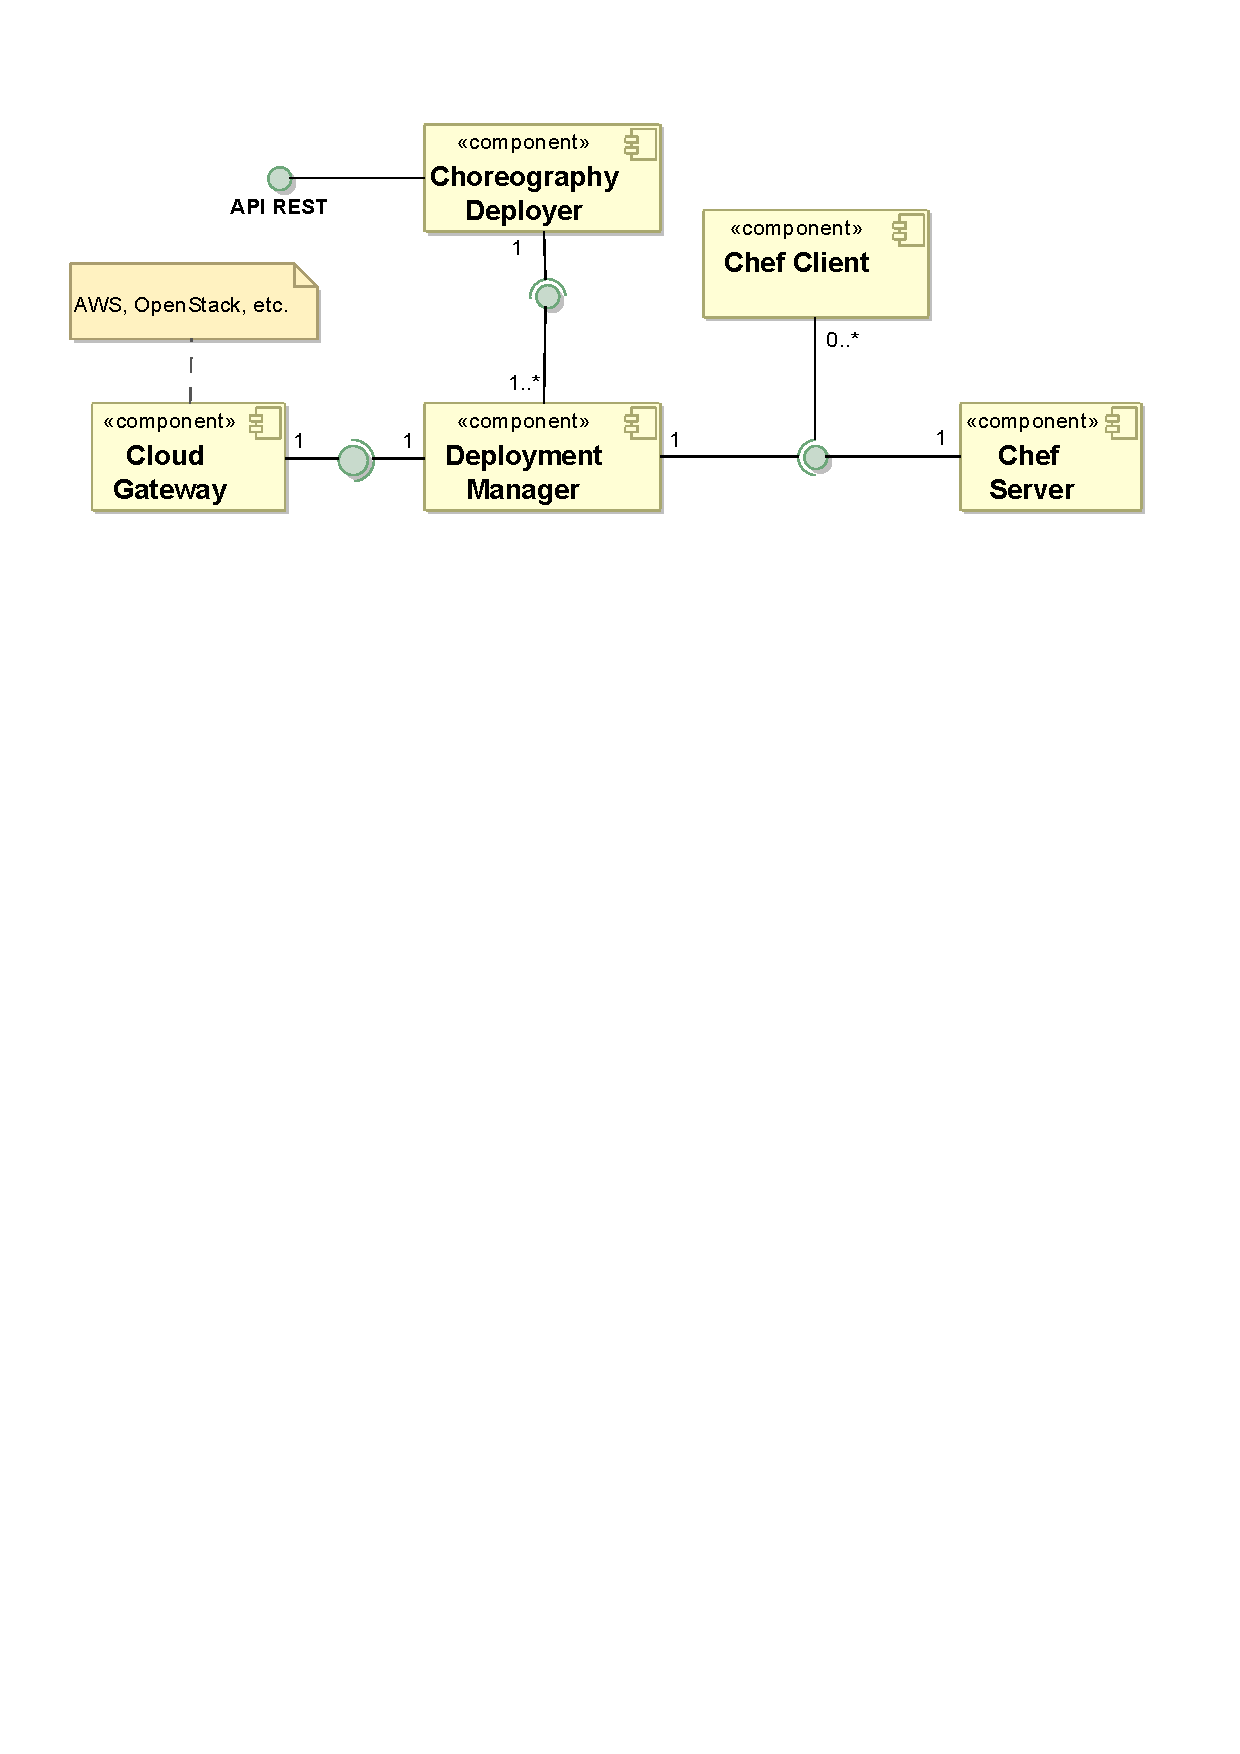
\includegraphics[width=.80\textwidth]{components.pdf} 
  \caption{Arquitetura do arcabouço \ee}
  \label{fig:ee_componentes} 
\end{figure}

\begin{description}

\item [Cloud Gateway:]

Este componente cria e destrói máquinas virtuais em uma infraestrutura de computação em nuvem. Neste contexto, essas máquinas virtuais são também chamadas \emph{nós}. Esse componente é utilizado pelo Deployment Manager, que decide quando criar ou destruir os nós. Uma instância do Deployment Manager é configurada de acordo com o Cloud Gateway a ser utilizado. Nativamente são utilizados como Cloud Gateway o serviço EC dos Web Services da Amazon ou uma instalação do OpenStack. Outras tecnologias de nuvem ou virtualização são utilizadas mediante extensão do Node Pool Manager.

\item [Chef Server:]

Em um sistema gerenciado pelo Chef, as configurações de software de um nó são especificadas por meio de ``receitas''. As receitas especificam configurações do sistema operacional (exemplo: instalar o pacote Java em um sistema Debian), instalação e configuração de middlewares (exemplo: instalar o Tomcat), assim como a instalação de um serviço final implantado sobre o middleware já configurado (exemplo: um web service). Essas receitas e as associações entre receitas e nós são armazenadas no Chef Server. Os operadores do Chef atualizam essas configurações diretamente pela interface gráfica do Chef Server ou pelo uso do Knife, uma ferramenta de linha de comando que se comunica com o Chef Server por meio de uma API REST. Na arquitetura do Chef, a máquina onde o operador utiliza o Knife é denominada ``workstation''. A arquitetura de um sistema gerenciado pelo Chef pode ser observada na Figura~\ref{fig:chef_arquitetura}.

\item [Chef Client:]

Em cada nó gerenciado pelo Chef é instalado um programa denominado Chef Client, que utiliza a API REST do Chef Server para obter as receitas relacionadas ao nó e assim atualizar suas configurações de software. O processo de instalação do Chef Client no nó é denominado ``bootstrap'', e é executado por meio de um comando do Knife, que se conecta por SSH na máquina para realizar a instalação do Chef Client e suas dependências.

\item [Deployment Manager:]

Implanta os serviços em um ambiente de nuvem associado a uma organização. Através de uma operação REST, o Deployment Manager recebe a especificação de um serviço e seleciona um nó adequado para sua implantação, possivelmente considerando os requisitos não-funcionais do serviço. O Deployment Manager converte a especificação recebida em uma receita Chef que implementa o processo de instalação do serviço. Após gerar a receita, o Deployment Manager a armazena no Chef Server e, também utilizando o Chef, cria uma associação entre essa receita e o nó selecionado. Utilizando outra operação REST do Deployment Manager pode-se requisitar que um determinado nó seja atualizado de acordo com as receitas a ele relacionadas. Essa divisão do processo em duas chamadas ao Deployment Manager é adotada para evitar a sobrecarga de execuções desnecessárias do Chef Client.

\item [Choreography Deployer:]

O Choreography Deployer expõe uma API REST de operações que automatizam a implantação de coreografias de serviços web. O cliente do Choreography Deployer fornece uma especificação declarativa da coreografia composta por uma descrição arquitetural da coreografia e da localização dos artefatos a serem implantados. Baseado nessa especificação, o Choreography Deployer coordena invocações aos Deployment Managers implantados nas diferentes organizações que participam da coreografia. Após a implantação dos serviços, para cada par de serviços que se comunicam na coreografia, o Choreography Deployer informa ao serviço consumidor a localização do serviço provedor.

\end{description}

\begin{figure}[!h]
  \centering
  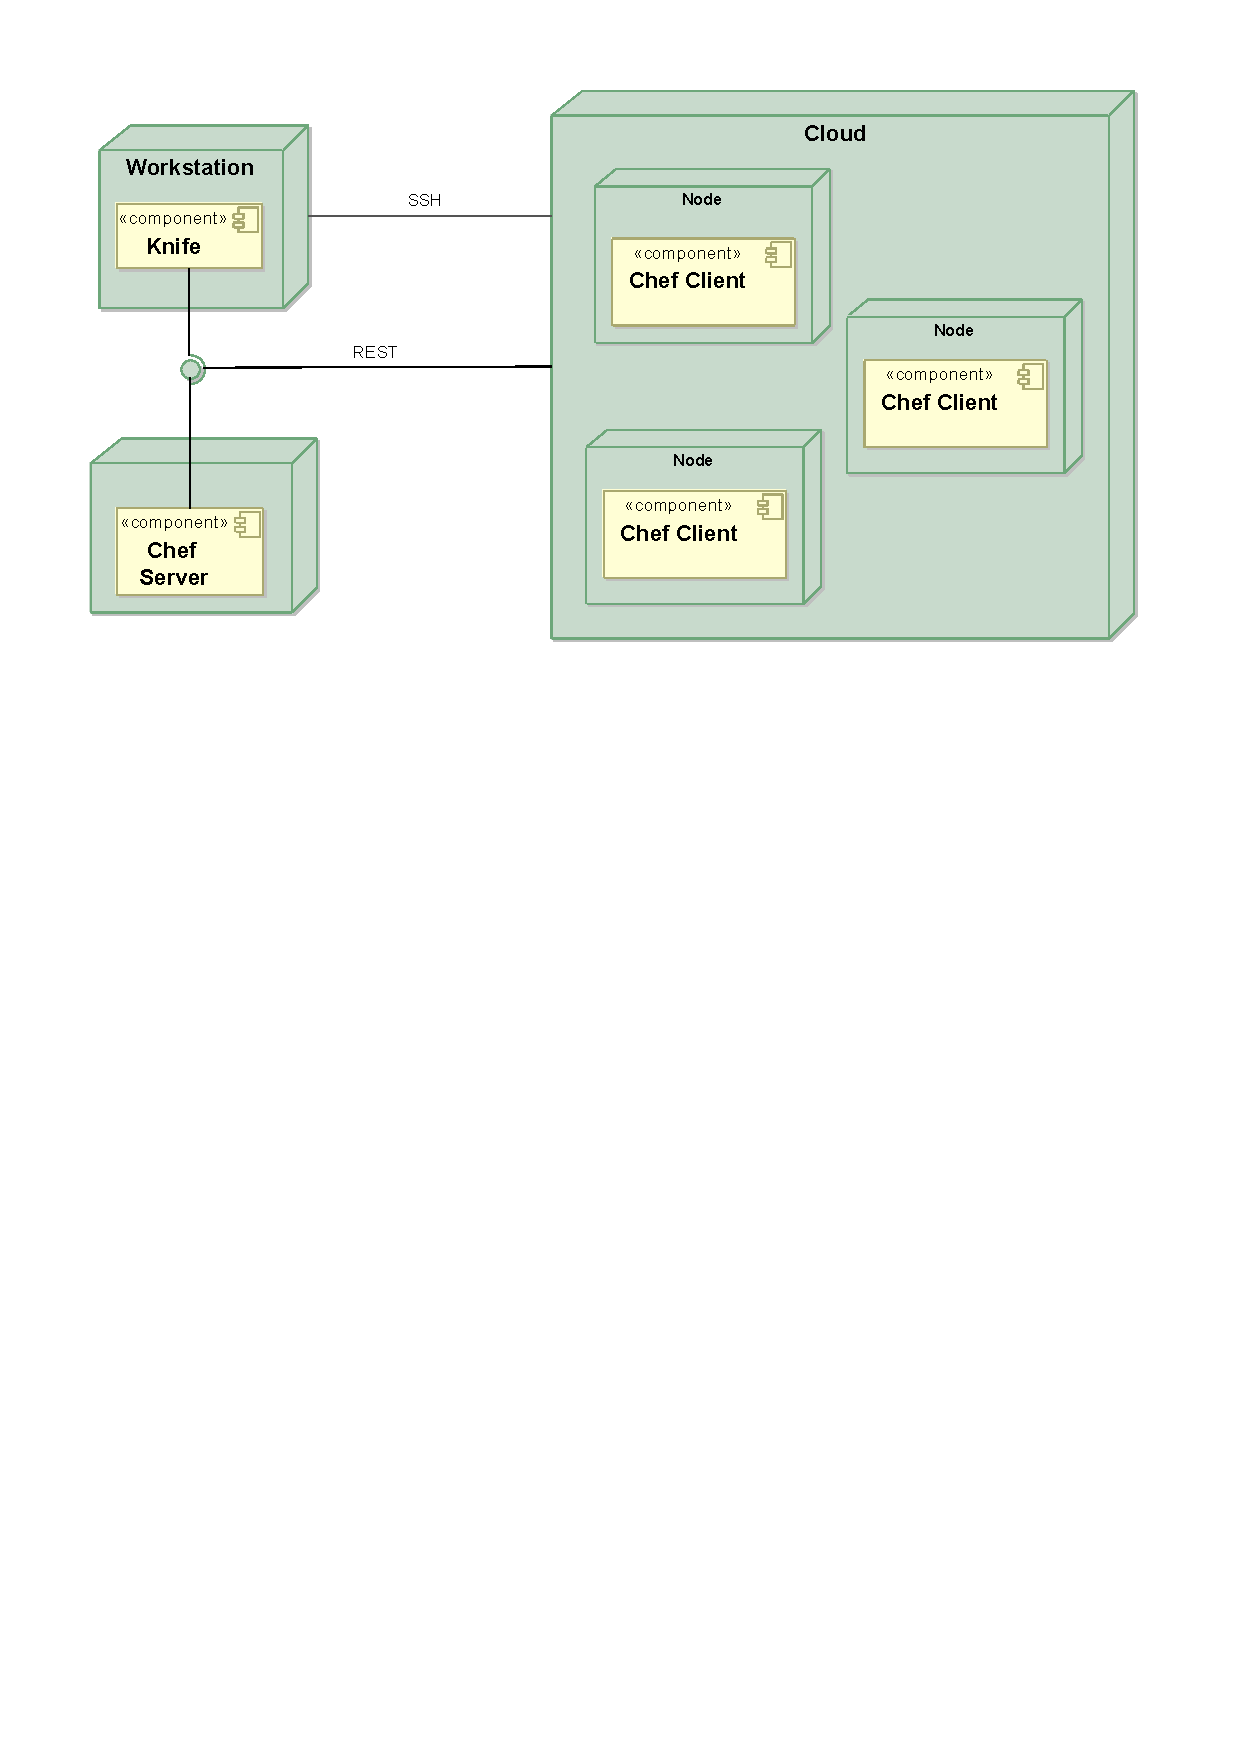
\includegraphics[width=.80\textwidth]{chef.pdf} 
  \caption{Arquitetura do Chef}
  \label{fig:chef_arquitetura} 
\end{figure}

A execução do Chef Client é demorada, tipicamente alguns minutos, dependendo do que está sendo instalado. Considerando que vários serviços podem ser implantados em um mesmo nó, a implantação da coreografia seria muito mais demorada caso cada invocação ao Deployment Manager resultasse em um pedido de atualização do nó onde o serviço deve ser implantado. Por isso, cabe ao Choreography Deployer a decisão de quando os nós são atualizados. Com isso, para cada nó, pode-se executar o Chef Client apenas uma vez para cada coreografia encenada. Essa otimização torna o sistema mais escalável. 

O diagrama de implantação da Figura~\ref{fig:ee_distribuicao} mostra como se distribuem os componentes do arcabouço Enactment Engine. Cada organização do diagrama está relacionada a uma instância de um sistema de nuvem privada (Open Stack, por exemplo), ou a uma conta de um provedor de nuvem pública (Amazon, por exemplo). A infraestrutura de cada organização deve possuir os seguintes componentes: um Cloud Gateway, um Chef Server e um Deployment Manager. 

\begin{figure}[!h]
  \centering
  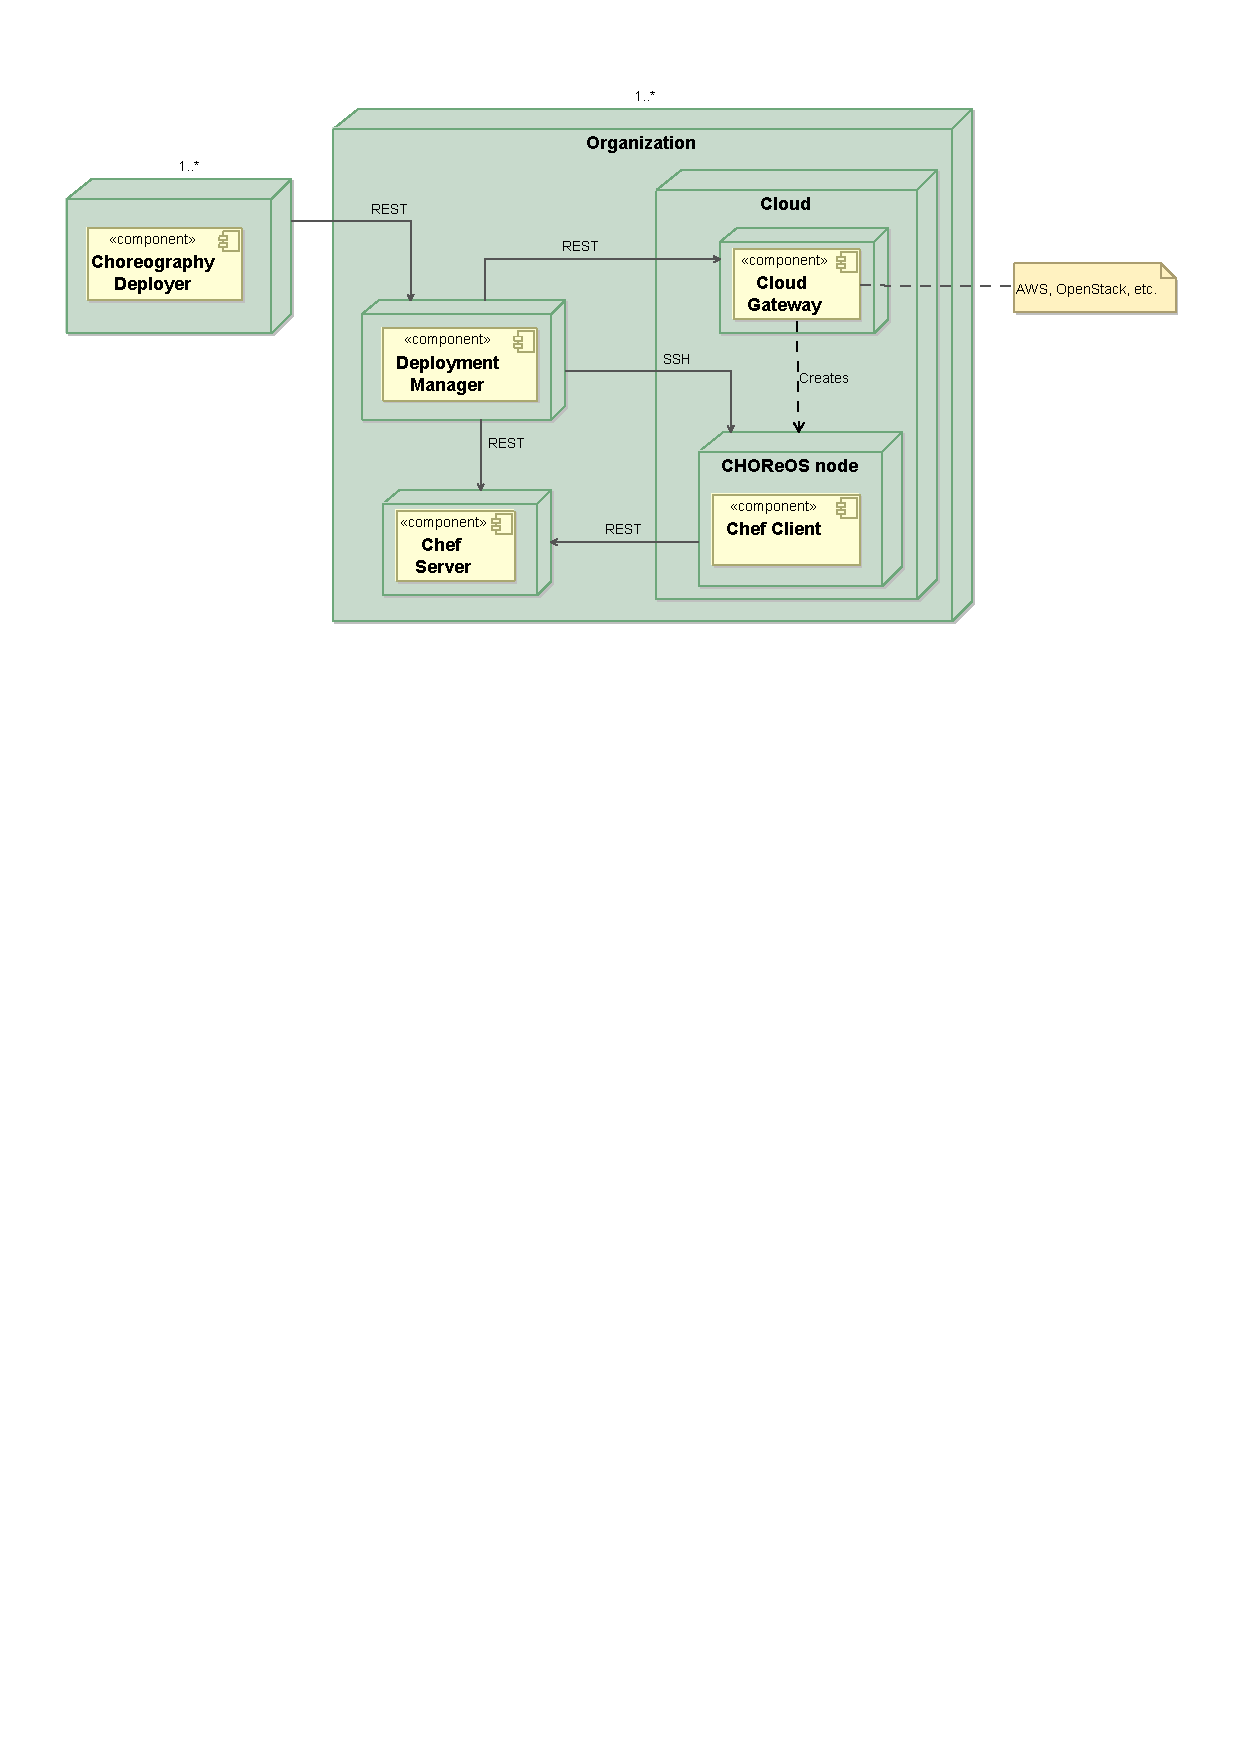
\includegraphics[width=1\textwidth]{ee_deployment.pdf} 
  \caption{Distribuição da implantação dos componentes do Enactment Engine}
  \label{fig:ee_distribuicao} 
\end{figure}

Um exemplo de ambiente distribuído com várias organizações é mostrado no diagrama da Figura~\ref{fig:ee_exemplo_distribuicao}. Nesse diagrama, existem três organizações: Linagora, Thales e USP. Cada organização corresponde ao nó ``organization'' do diagrama genérico de implantação (Figura~\ref{fig:ee_distribuicao}). Esse último diagrama também destaca o fato de que organizações podem tanto usar suas próprias nuvens privadas, quanto alguma nuvem pública, como a da Amazon. Caso uma organização deseje utilizar mais de um sistema de nuvem, ela deverá ser modelada em nosso arcabouço como várias organizações diferentes. Por exemplo, se a organização USP deseja utilizar uma nuvem privada com o OpenStack e o serviços da Amazon, pode-se modelar as seguintes organizações: USP\_OpenStack e USP\_AWS.

\begin{figure}[!h]
  \centering
  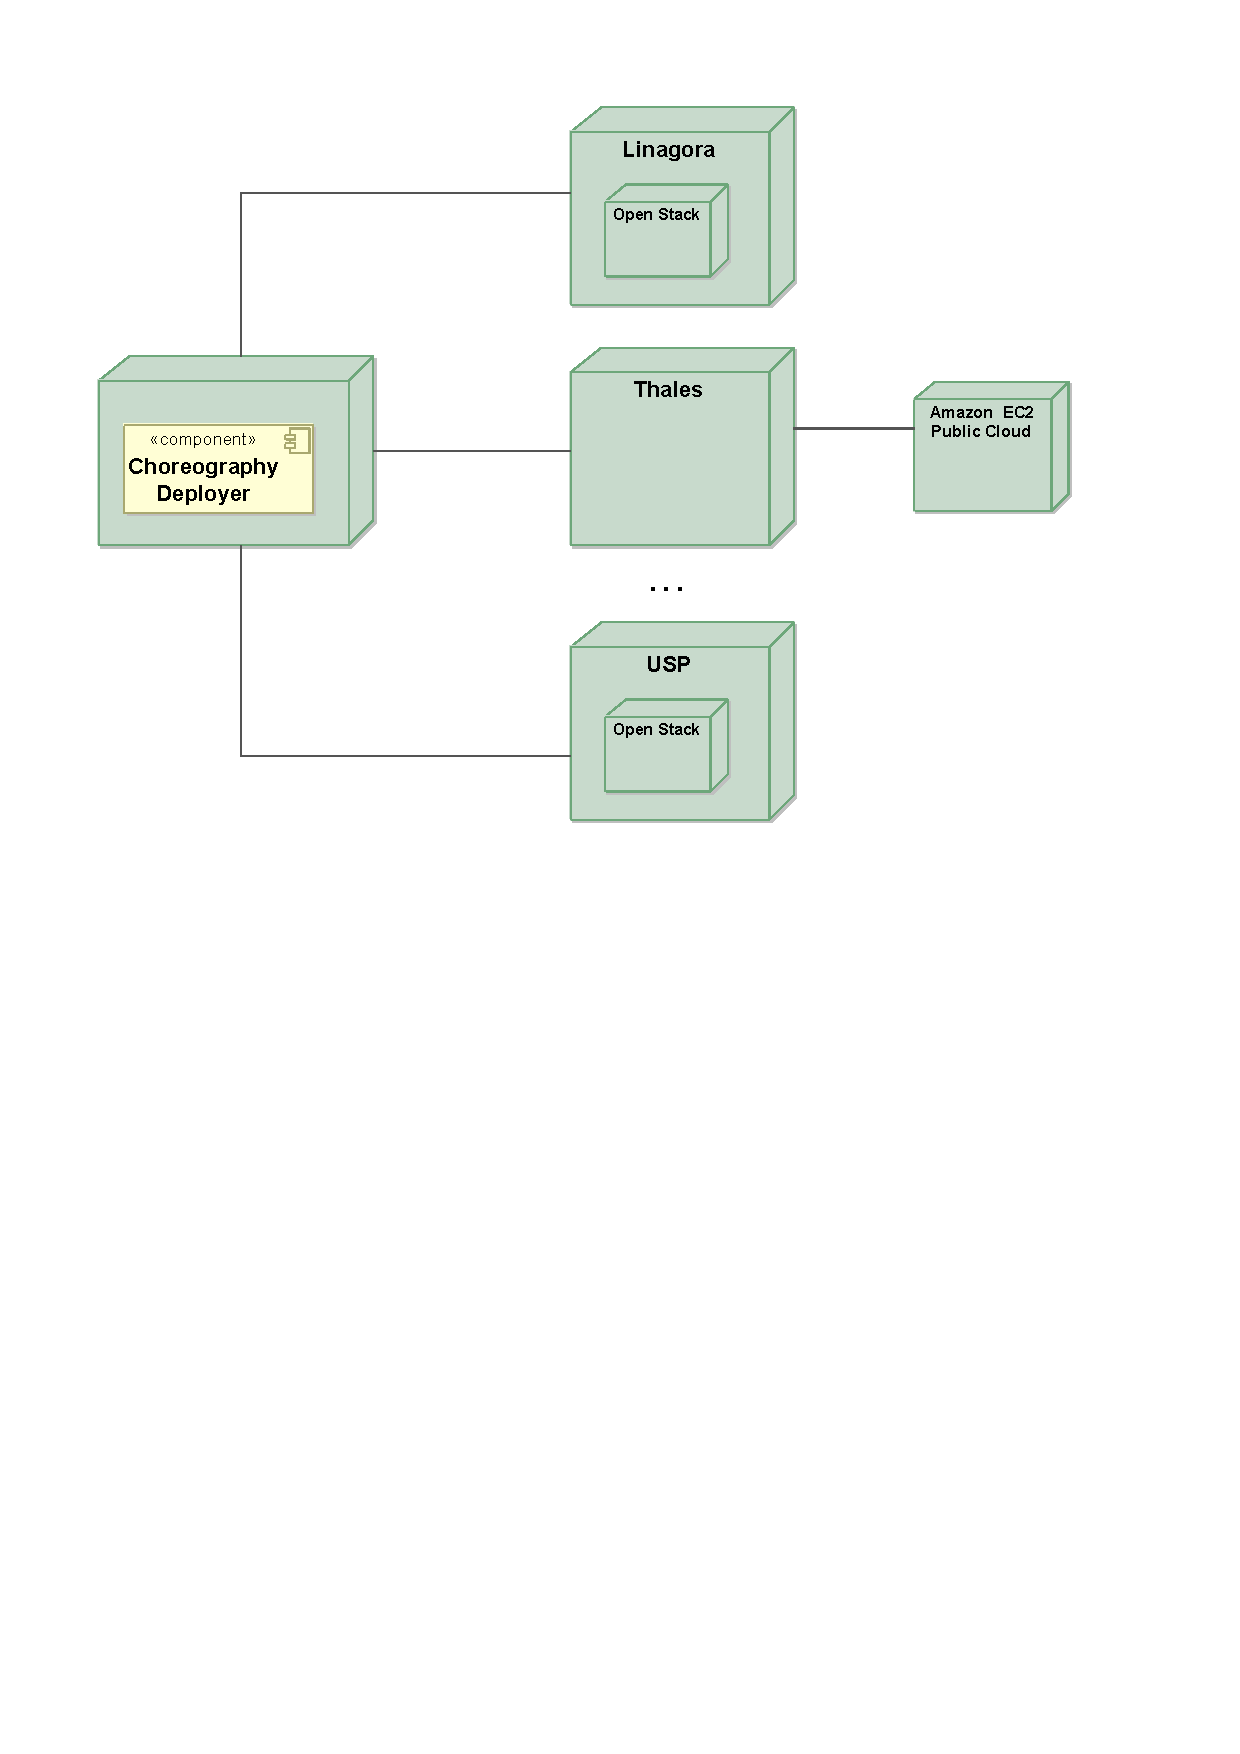
\includegraphics[width=.80\textwidth]{ee_exemplo_distribuicao.pdf} 
  \caption{Exemplo de uso do Enactment Engine em diferentes organizações}
  \label{fig:ee_exemplo_distribuicao} 
\end{figure}

Terminamos esta seção com um diagrama de sequência (Figura~\ref{fig:ee_sequencia}) que evidencia detalhes da interação entre os componentes do arcabouço. Esse diagrama ilustra o processo de encenação de uma pequena coreografia de dois serviços, na qual o serviço A é consumidor do serviço B.

\begin{figure}[!h]
  \centering
  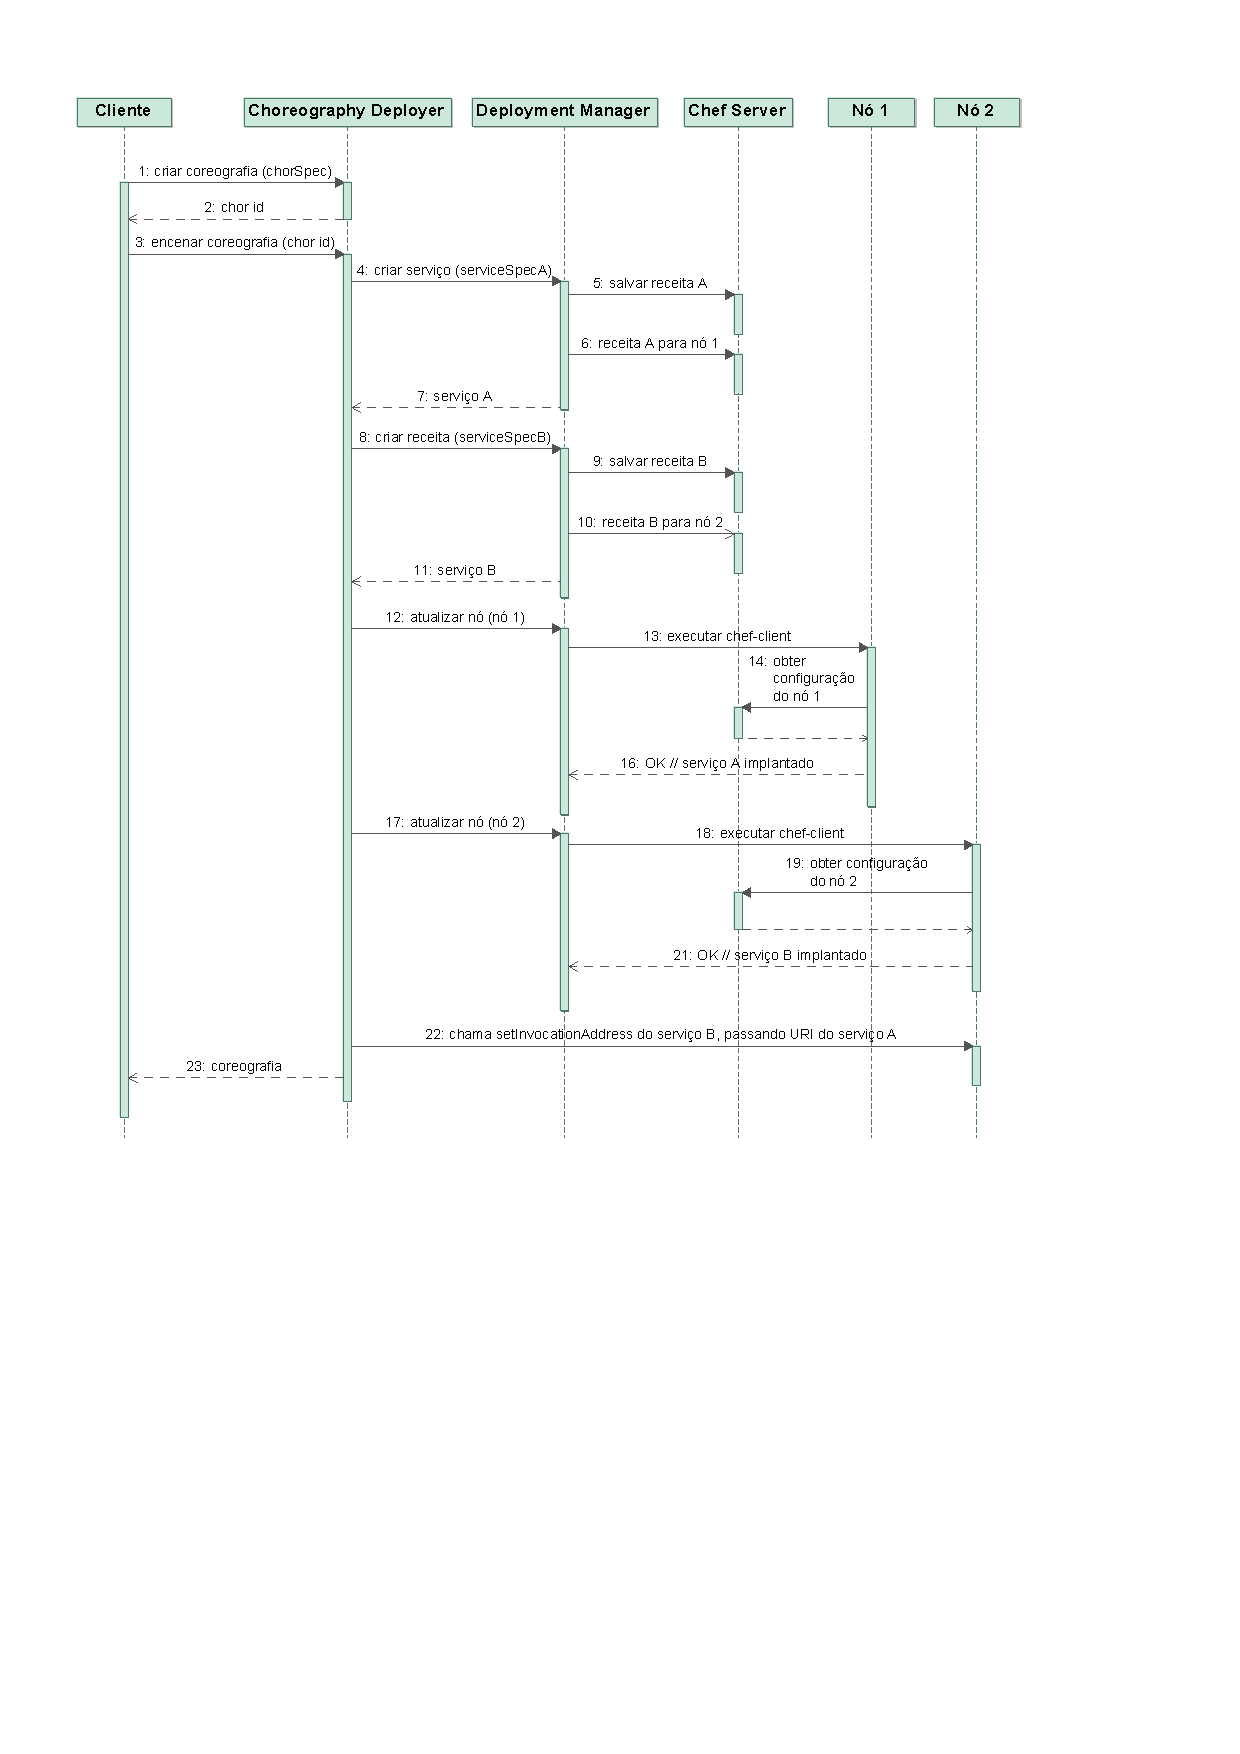
\includegraphics[width=.80\textwidth]{sequence.pdf} 
  \caption{Exemplo de implantação de uma coreografia de dois serviços}
  \label{fig:ee_sequencia} 
\end{figure}

O processo de implantação se inicia com duas requisições ao Choreography Deployer: uma para a criação do recurso\footnote{Usamos aqui o termo ``recurso'' em seu sentido usual em arquiteturas REST.} \emph{coreografia} associado à especificação fornecida pelo cliente e outra para a encenação da coreografia. Para cada especificação de serviço contido na especificação da coreografia, o Choreography Deployer requisita a criação de um recurso \emph{serviço} ao Deployment Manager. Para isso, o Deployment Manager cria uma receita Chef que automatiza a instalação do serviço, armazena-a no Chef Server e associa a receita a algum nó por ele selecionado. O Deployment Manager retorna ao Choreography Deployer o recurso \emph{serviço}, contendo a URI de acesso a esse serviço e uma referência ao nó selecionado. Em seguida, o Choreography Deployer requisita ao Deployment Manager a atualização de todos os nós selecionados. Quando o Deployment Manager recebe um pedido de atualização de nó, ele se conecta por SSH a esse nó e executa o Chef Client, que se comunica com o Chef Server para obter as receitas associadas àquele nó e instalar os serviços com base nas receitas obtidas. O Choreography Deployer ainda invoca a operação \emph{setInvocationAddress} do serviço B, informando ao serviço B a URI de acesso do serviço A. Finalmente, o Choreography Deployer devolve ao cliente a representação da coreografia, contendo informações da implantação, especialmente as URIs dos serviços em execução.

Uma observação sobre o diagrama da Figura~\ref{fig:ee_sequencia} é que todas as operação foram dispostas de forma sequencial para facilitar a leitura do diagrama, mas o Choreography Deployer realiza as chamadas de criação dos serviços em paralelo, assim como as chamadas de atualização dos nós e as invocações às operações \emph{setInvocationAddress}.

\section{Descrição arquitetural da coreografia}
\label{sec:adl}

O Enactment Engine recebe de seus clientes a especificação da coreografia na forma de uma descrição arquitetural com as informações necessárias e suficientes para que se possa realizar a implantação da coreografia. O Enactment Engine também devolve ao seu cliente informações sobre a implantação da coreografia, em especial as localizações de acesso aos serviços. Essa descrição da coreografia consiste em uma Linguagens de Descrição Arquitetural, como a dos trabalhos vistos no Capítulo~\ref{cap:relacionados}. A nossa ADL consiste na descrição de objetos relacionados entre si seguindo a estrutura de classes apresentada na Figura~\ref{fig:ee_adl}. Em nossa implementação, essa descrição é realizada com representações em XML, que são trocadas entre o Enactment Engine e seu cliente. O Apêndice~\ref{ape:xml} lista exemplos de entrada e de saída em XML do Enactment Engine, bem como o \emph{schema} que define a formatação dos dados em XML.  

\begin{figure}[!h]
  \centering
  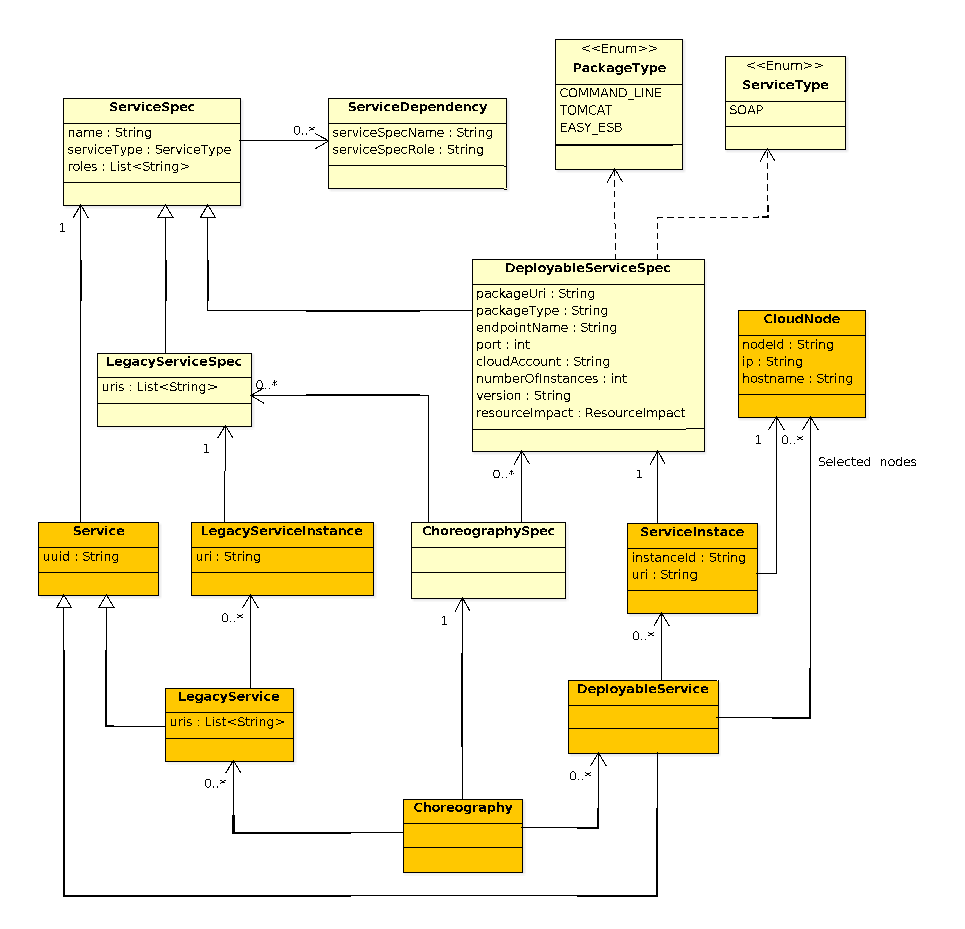
\includegraphics[width=.80\textwidth]{adl.pdf} 
  \caption{Estrutura da descrição arquitetural de uma coreografia}
  \label{fig:ee_adl} 
\end{figure}

Apresentaremos agora uma breve descrição sobre cada uma das classes apresentadas no diagrama.

\begin{description}

\item [ServiceSpec:] especificação de um serviço com informações necessárias para que se realize a implantação de um serviço fora do contexto da coreografia.

\item [ServiceDependency:] representa uma dependência entre serviços. Se o serviço A invoca o serviço B, então o serviço A depende do serviço B.

\item [ChorServiceSpec:] especificação de um serviço com informações necessárias para que se realize a implantação de um serviço em uma coreografia.

\item [ChorSpec:] Uma coleção de elementos ChorServiceSpec que especificam uma coreografia.

\item [Service:] contém informações sobre um serviço já implantado.

\item [Choreography:] contém informações sobre os serviços implantados que formam uma coreografia.

\end{description}

Iremos agora detalhar o significado dos atributos das classes já apresentadas:

\begin{description}

\item [Service.name e ServiceSpec.name:] um nome único para o serviço dentro da coreografia.

\item [ChorServiceSpec.owner:] organização que controla a infraestrutura onde o serviço deve ser implantado. Com esse atributo pode-se garantir que serviços sejam instalados em organizações de confiança do fornecedor do serviço, assim como proposto por Watson~\cite{Watson2006Dynasoar}.

\item [ChorServiceSpec.group:] dois serviços especificados no mesmo grupo devem ser implantados no mesmo nó.

\item [ChorServiceSpec.roles:] lista de papéis desempenhados pelo serviço.

\item [ServiceSpec.type:] especifica o tipo de serviço, de acordo com a enumeração ServiceType, que contém os valores SOAP e REST. Com essa informação, o Enactment Engine sabe como acessar a operação setInvocationAddress desses serviços, para que os serviços da coreografia saibam da localização uns dos outros. 

\item [ServiceSpec.artifactType:] o tipo do artefato implantável. Deve corresponder a algum valor da enumeração ArtifactType. Se tipo do artefato for COMMAND\_LINE, o serviço é iniciado com o comando ``java -jar''. Se possui o valor TOMCAT, é simplesmente instalado em um Tomcat em execução. Se for EASY\_ESB, assume-se que se trata de um arquivo de configuração que executará ações em um nó do EasyESB. Se for LEGACY, trata-se de um serviço já acessível pela Internet.

\item [ServiceSpec.codeUri:] a localização do artefato que instalará o serviço. Se o tipo do serviço é LEGACY o valor de codeUri corresponde à URI do serviço já disponível.

Para o artefato COMMAND\_LINE, o atributo codeUri pode apontar para um arquivo jar ou para um tar.gz, que deve ter um jar compactado em sua raiz. O suporte à opção tar.gz é muito importante para que o cliente mantenha a separação entre código executável e configuração de seus serviços. Caso apenas os arquivos jars fossem suportados, o cliente seria obrigado a empacotar as configurações de seu serviço dentro do próprio jar, o que é visto como uma má prática no livro Continous Delivery~\cite{Humble2011Continuous}, que prega que um binário deve ser executável, na medida do possível, em todos os ambientes necessários. Ou seja, gerar um executável para cada plataforma alvo é indesejável. Esse objetivo pode ser atingido com a separação das configurações específicas de cada ambiente em arquivos de configuração. Infelizmente, tal prática não é viável para artefatos do tipo war, que são implantados no Tomcat.

\item [ServiceSpec.port:] a porta TCP utilizada pelo serviço. Obrigatório caso o tipo seja COMMAND\_LINE.

\item [ServiceSpec.endpointName:] o sufixo do endpoint do serviço após sua implantação. Por exemplo, se o serviço é implantado e acessível pela URI http://<IP>:<PORTA>/choreos/service, o endpointName é a string ``choreos/service''. Se o tipo é LEGACY, então endpointName é vazio.

\item [ServiceSpec.version:] a versão do serviço, que será usada pela operação de atualização da coreografia para determinar os serviços que precisam ser re-implantados.

\item [ServiceSpec.resourceImpact:] conjunto de pares chave-valor que especificam os requisitos não-funcionais do serviço. Esses requisitos não-funcionais são utilizados pelo Node Pool Manager para a escolha, se possível, de um nó nuvem que satisfaça esses requisitos.

\item [Service.uri:] URI completa do serviço implantado.

\item [Service.hostname:] hostname do nó em que o serviço foi implantado.

\item [Service.ip:] IP público do nó em que o serviço foi implantado.

\item [Service.nodeId:] ID do nó onde o serviço foi implantado. Este ID possibilita acessar mais informações sobre o nó pelo Node Pool Manager. 

\end{description}

Segundo Dearle~\cite{Dearle2007PastPresentFuture}, componentes podem ser ligados entre si em vários momentos: compilação, montagem, configuração e execução. Em nosso contexto, a ligação deve ser efetuada necessariamente em tempo de execução, pois é somente nesse momento que teremos os endereços completos dos serviços implantados. Uma das possibilidades apontadas por Dearle para efetivação da ligação em tempo de execução é a utilização do padrão de injeção de dependência, conforme introduzido por Fowler~\cite{Fowler2004Inversion}. A injeção de dependências é utilizada em contêineres como o Springer\footnote{\url{http://www.springer.org}}, no qual o middleware passa ao componente referências de suas dependências. No entanto, Dearle ainda alega que há uma falta de arcabouços para a aplicação da injeção de dependência de forma distribuída.

A solução adotada no \ee\ para possibilitar a ligação entre serviços envolve a utilização do middleware para a passagem de endereços dos serviços implantados aos seus consumidores, o que é feito com base na lista de objetos \textsf{ServiceDependency} pertencentes a um \textsf{ChorServiceSpec}. Essa solução consiste na aplicação do padrão de injeção de dependência de forma distribuída, e é similar ao que foi feito nos trabalhos sobre a linguagem Darwin~\cite{Magee1996Dynamic, Magee1994Regis}. Para que esse processo funcione, é preciso que cada serviço na coreografia que possua dependências implemente uma operação denominada \emph{setInvocationAddress}, por nós padronizada. Essa operação recebe como argumentos as seguintes informações sobre a dependência: papel do serviço, nome do serviço no contexto da coreografia e a URI de acesso ao serviço.  Em uma coreografia em que, por exemplo, um serviço de agência de viagem dependa do serviço de uma companhia aérea, o \ee\ poderá executar a seguinte invocação ao serviço da agência de viagens: \texttt{setInvocationAddress('Companhia Aérea', 'Nimbus Airline', 'http://192.168.56.107:8080/nimbus/ws/')}. Nessa solução, a ``inteligência'' em determinar quais serviços satisfazem as necessidades de outros serviços está na camada que produz a entrada do \ee.

Apesar dos benefícios de uma solução como essa, Dearle~\cite{Dearle2007PastPresentFuture} também alerta sobre a desvantagem em forçar componentes a aderirem convenções de codificação impostas pelo middleware, o que poderia restringir o serviço a uma determinada linguagem de programação ou a algum middleware específico. Reconhecemos que esse problema existe em nossa solução, mas acreditamos que o desenho adotado ameniza os problemas levantados, pois tudo o que o serviço é obrigado a fazer é implementar a operação \texttt{setInvocationAddress} e conhecer os papeis de suas dependências, o que implica em conhecer a interface sintática de cada papel. Dessa forma, nossa solução não restringe o serviço a nenhuma linguagem e possibilita seu uso por outros middlewares que adotem a mesma convenção para o \texttt{setInvocationAddress}.

\section{Interface}
\label{sec:interface}

Os sistemas externos ao Enactment Engine utilizam suas funcionalidades por meio da API REST exposta pelo componente Choreography Deployer, que é descrita nesta subseção. Por se tratar de uma API REST, o cliente pode ser implementado em qualquer linguagem e ambiente que possua alguma biblioteca HTTP. Também disponibilizamos um cliente na forma de uma biblioteca na linguagem Java, tornando o uso do Enactment Engine ainda mais simples para os usuários da linguagem Java, atualmente uma das mais utilizadas do mercado. Seguimos agora listando as operações disponíveis. 

\begin{description}

\item [Criar coreografia:]

Descrição: registra a especificação de uma coreografia no Choreography Deployer. Essa especificação é a descrição arquitetural da coreografia, estruturada de acordo com a classe ChorSpec. Esa operação não realiza a encenação da coreografia.

%Requisição:
%URI: choreographydeployer/chors
%Método: POST
%Corpo: representação XML da classe ChorSpec.
%
%Resposta em caso de sucesso:
%Código de estado: 201 CREATED
%Cabeçalho ?location?: choreographydeployer/chors/{id} 
%
%Respostas em caso de falha:
%400 BAD REQUEST
%500 INTERNAL SERVER ERROR

{\small
\begin{tabular}{|c|c|c|c|}
\hline 
\itshape{Método HTTP} & \itshape{URI} & \itshape{Corpo da requisição} & \itshape{Respostas} \\ 
\hline 
POST & /chors & 

\begin{minipage}{2in}
Representação XML \\ de \textsf{ChorSpec}\\ 
(ver Listagem \ref{lst:chor_spec_xml})
\end{minipage} 
&

\begin{minipage}{2in}
\begin{verbatim}

201 CREATED
location = "/chors/{id}"

400 BAD REQUEST

500 ERROR

\end{verbatim}
\end{minipage} 
\\ 
\hline 
\end{tabular} 
}

\item [Obter coreografia:]

Obtém informações sobre uma coreografia registrada no Choreography Deployer. Essas informações se referem à especificação da coreografia e ao estado da implantação de seus serviços, como os nós em que os serviços foram implantados, no caso de a implantação já ter sido realizada.

%Requisição:
%URI: choreographydeployer/chors/{id}
%Método: GET
%
%Resposta em caso de sucesso:
%Código de estado: 200 OK
%Cabeçalho ?location?: choreographydeployer/chors/{id} 
%Corpo: representação em XML da classe Choreography. 
%
%Respostas em caso de falha:
%400 BAD REQUEST
%404 NOT FOUND
%500 INTERNAL SERVER ERROR

{\small
\begin{tabular}{|c|c|c|c|}
\hline 
\itshape{Método HTTP} & \itshape{URI} & \itshape{Corpo da requisição} & \itshape{Respostas} \\ 
\hline 
GET & /chors/\{id\} & - &
\begin{minipage}{2in}
\begin{verbatim}

200 OK
location = "/chors/{id}"
Corpo: 
\end{verbatim}
Representação XML \\ de \textsf{Choreography}\\ 
(ver Listagem \ref{lst:chor_xml})

\begin{verbatim}
400 BAD REQUEST

404 NOT FOUND

500 ERROR

\end{verbatim}
\end{minipage} 
\\ 
\hline 
\end{tabular}
}

\item [Encenar coreografia:]

Descrição: realiza a encenação de uma coreografia já registrada no Choreography Deployer. Ao fim do processo, detalhes do resultado da implantação são retornados na representação XML da coreografia. A implementação dessa operação deve possuir duas importantes propriedades: 1) a falha na encenação de parte da coreografia não deve interromper o encenação do resto da coreografia; 2) a operação deve ser \emph{idempotente}, ou seja, uma nova requisição para a encenação da mesma coreografia não deve tentar implantar os serviços já implantados, mas somente aqueles cujas implantações falharam na última execução. Para que serviços sejam atualizados, é preciso utilizar um novo valor no atributo ``versão'' da especificação do serviço.

%Requisição:
%URI: choreographydeployer/chors/{id}/enactment
%Método: POST
%
%Resposta em caso de sucesso:
%Código de estado: 200 OK
%Cabeçalho ?location?: choreographydeployer/chors/{id} 
%Corpo: representação em XML da classe Choreography. 
%
%Respostas em caso de falha:
%400 BAD REQUEST
%404 NOT FOUND
%500 INTERNAL SERVER ERROR

{\small
\begin{tabular}{|c|c|c|c|}
\hline 
\itshape{Método HTTP} & \itshape{URI} & \itshape{Corpo da requisição} & \itshape{Respostas} \\ 
\hline 
POST & /chors/\{id\}/enactment & - &
\begin{minipage}{2in}
\begin{verbatim}

200 OK
location = "/chors/{id}"
Corpo: 
\end{verbatim}
Representação XML \\ de \textsf{Choreography}\\ 
(ver Listagem \ref{lst:chor_xml})

\begin{verbatim}
400 BAD REQUEST

404 NOT FOUND

500 ERROR

\end{verbatim}
\end{minipage} 
\\ 
\hline 
\end{tabular} 
}

\item [Atualizar coreografia:]

Registra uma nova versão de uma coreografia no Choreography Deployer. Os serviços atualizados na nova versão da coreografia devem possuir um novo número de versão em suas especificações. Essa operação, assim como a criação da coreografia, não encena a nova coreografia. Para isso, é preciso invocar novamente a operação de encenação.

%Requisição:
%URI: choreographydeployer/chors/{id}
%Método: PUT
%Corpo: representação em XML da classe ChorSpec
%
%Resposta em caso de sucesso:
%Código de estado: 200 OK
%Cabeçalho ?location?: choreographydeployer/chors/{id} 
%Corpo: representação em XML da classe Choreography. 
%
%Respostas em caso de falha:
%400 BAD REQUEST
%404 NOT FOUND
%500 INTERNAL SERVER ERROR

{\small
\begin{tabular}{|c|c|c|c|}
\hline 
\itshape{Método HTTP} & \itshape{URI} & \itshape{Corpo da requisição} & \itshape{Respostas} \\ 
\hline 
PUT & /chors/\{id\} & 

\begin{minipage}{2in}
Representação XML \\ de \textsf{ChorSpec}\\ 
(ver Listagem \ref{lst:chor_spec_xml})
\end{minipage} 
&
\begin{minipage}{2in}
\begin{verbatim}

200 OK
location = "/chors/{id}"
Corpo: 
\end{verbatim}
Representação XML \\ de \textsf{Choreography}\\ 
(ver Listagem \ref{lst:chor_xml})

\begin{verbatim}
400 BAD REQUEST

404 NOT FOUND

500 ERROR

\end{verbatim}
\end{minipage} 
\\ 
\hline 
\end{tabular} 
}

Em nosso trabalho a atualização dos serviços será feita da forma mais simples possível: apenas substituindo o serviço existente por sua nova versão. Contudo, tal procedimento pode provocar falhas na comunicação entre os serviços de uma coreografia. Vários trabalhos \cite{Kramer1990Philosophers, Vandewoude2007Tranquility, Xiaoxing2011VersionConsistent} estudam o processo de atualização dinâmica, pelo qual as conversações correntes são preservadas durante a atualização de um serviço. Embora não esteja no escopo de nosso trabalho, acreditamos que a arquitetura do \ee\ possa ser evoluída para que a operação de atualização de coreografia utilize procedimentos seguros de atualização dinâmica, dentre os quais destacamos a proposta de Xiaoxing et al~\cite{Xiaoxing2011VersionConsistent}.

\end{description}

\section{Pontos de extensão}
\label{sec:extensao}

Para lidar com as particularidades do ambiente de cada organização, o Enactment Engine fornece alguns pontos de extensão. Esses pontos de extensão são classes que desenvolvedores devem escrever na linguagem Java e que, de acordo com as configurações do sistema, poderão ser executadas por nossa plataforma.

\begin{description}

\item [CloudProvider:] 

Implementando a interface CloudProvider é possível o suporte a novas plataforma de computação em nuvem. Atualmente nossa implementação suporta o serviço EC2 do AWS e o OpenStack.

\begin{lstlisting}[frame=trbl, label=lst:cloud_provider, caption=Interface CloudProvider]
/**
 * Provides access to cloud service functions to create nodes on the cloud. 
 * 
 * Each specific provider (e.g. AmazonWS) must have an implementing class of this interface.
 * 
 * 
 */
public interface CloudProvider {

	public String getproviderName();
	
	public Node createNode(Node node) throws RunNodesException;

	public Node getNode(String nodeId) throws NodeNotFoundException;

	public List<Node> getNodes();

	public void destroyNode(String id) throws NodeNotDestroyed, NodeNotFoundException;

	public Node createOrUseExistingNode(Node node) throws RunNodesException;

}
\end{lstlisting}


\item [NodeSelector:]

A implementação da interface NodeSelector define uma nova política de alocação de serviços em nós da nuvem, que pode levar em conta os requisitos não-funcionais do serviço e propriedades dos nós à disposição.

\begin{lstlisting}[frame=trbl, label=lst:node_selector, caption=Interface NodeSelector]
/**
 * Selects a node to apply a given configuration
 * 
 * The selection can consider functional requirements, which is provided by config.name and non-functional requirements, which is provided by config.resourceImpact
 * Implementing classes must receive a CloudProvider
 * 
 * @author leonardo
 *
 */
public interface NodeSelector {

	public Node selectNode(Config config);
}
\end{lstlisting}

Formas similares dessa funcionalidade são também utilizadas em estudos já apresentados na seção de trabalhos relacionados.  O trabalho de Magee e Kramer~\cite{Magee1997Corba} apresenta a seleção de nós em função da utilização de CPUs nos nós existentes, não havendo possibilidade de utilização de outros critérios, como memória, disco, custo etc. Nos sistemas apresentados por Dolstra et al.~\cite{Dolstra2005Configuration} e Balter et al.~\cite{Balter1998Olan} é preciso que a distribuição dos serviços seja especificada com o uso dos IPs das máquinas nas quais os serviços devem ser implantados, o que não é possível em um ambiente de nuvem. Por fim, o \emph{broker} apresentado por Watson et al. é o componente que mais se assemelha ao nosso NodeSelector, pois os autores deixam claro que várias implementações diferentes são possíveis, considerando-se diferentes tipo de requisitos e diferentes fontes de monitoramento. Como a escolha é feita em tempo de execução do serviço, seria também possível uma seleção que independa de IPs estabelecidos em tempo de projeto. No entanto, os autores não explicam como os usuários de seu sistema, os provedores de infraestrutura, deveriam proceder para criar seus próprios \emph{brokers} personalizados.

Para avançar em relação às limitações dos trabalhos anteriormente citados,  consideramos como requisitos principais a dinamicidade do ambiente de nuvem, que nos impede de conhecer os IPs das máquinas em tempo de configuração, bem como a flexibilidade para que cada organização determine os requisitos de distribuição dos serviços.

\item [Receitas:]

Um serviço pode ser distribuído por diferentes tipos de artefatos implantáveis, como em um JAR ou em um WAR, por exemplo. Como existem muitas outras opções, é preciso que esse seja um ponto de flexibilidade. Para cada tipo de distribuição, pode-se escrever uma receita Chef que sabe como instalar e executar o serviço. Como essas receitas são criadas dinamicamente com base em modelos pré-definidos e propriedades do serviço a ser implantado, é preciso também implementar a interface RecipeBuilder para criar uma nova extensão correspondente a um novo tipo de artefato implantável.

\begin{lstlisting}[frame=trbl, label=lst:recipe_builder, caption=Interface RecipeBuilder]
public interface RecipeBuilder {
	
 /**
  * Uses the template to create a new recipe according to service specification.
  * This new recipe can be used by Chef to deploy the service.
  * 
  * @param service
  * @return
  */
 public Recipe createRecipe(ServiceSpec serviceSpec);
}
\end{lstlisting}

\item [ContextSender:]

A ligação entre serviços de uma coreografia depende da passagem de endereços que é feita do Choreography Deployer para os serviços. Para isso, o Choreography Deployer precisa invocar a operação setInvocationAddres dos serviços. A implementação de tal invocação se dará de forma diferente se o serviço for SOAP ou REST. A implementação da interface ContextSender possibilita ao Choreography Deployer realizar a invocação da operação setInovcationAddress em serviços de outras tecnologias (JMS e CORBA por exemplo). Nota-se que para cada um desses tipos de serviços adicionados pelo usuário, é preciso criar uma convenção para a assinatura sintática da operação setInvocationAddres.

\begin{lstlisting}[frame=trbl, label=lst:context_sender, caption=Interface ContextSender]
public interface ContextSender {
	
 /**
  * Calls setInvokationAddress operation on service in the serviceEndpoint.
  * So, the service in endpoint will know that its
  * partner with partnerRole is realized by partnerEndpoint.
  * 
  * @param serviceEndpoint
  * @param partnerRole
  * @param partnerEndpoint
  * @throws ContextNotSentException if context was not successfully set
  */
  public void sendContext(String serviceEndpoint, String partnerRole, String partnerEndpoint) throws ContextNotSentException;

}
\end{lstlisting}

\end{description}

\section{Aspectos de grande escala}
\label{sec:solucao_grande_escala}

\fabio{Fazer uma tabela de características, mostrando quais suportamos e quais não. Se der, comparar com outros trabalhos}

Na seção ``Computação em Grande Escala'' abordamos alguns desafios, práticas e princípios necessários para a construção de sistemas de grande escala. Dado que nossa arquitetura deve possibilitar a implantação de sistemas de grande escala, relatamos nesta seção quais práticas levamos em consideração na definição de nossa arquitetura, assim como limitações de nossa arquitetura devido a outras práticas não adotadas.

O princípio adotado mais importante é o de fornecer uma ferramenta que possibilite um processo totalmente automatizado para a implantação de coreografias. Contudo, cabe ressaltar que um processo totalmente automatizado não depende apenas do Enactment Engine. Por exemplo, o Enactment Engine deve receber como entrada um XML que descreva a coreografia. Espera-se que esse XML seja gerado automaticamente de alguma forma, mas essa é uma responsabilidade além do escopo de nossa proposta, de forma que na prática nosso sistema também funcionaria com um XML gerado manualmente. No contexto do projeto CHOReOS, essa especificação é gerada por um processo automático de síntese que recebe como entrada a especificação da coreografia na notação BPMN2~\cite{Autili2013Synthesis}.

Buscando a simplicidade, adotamos REST como o estilo de serviços oferecidos pela nossa arquitetura. Isso evita algum overhead que seria gerado pelo SOAP, possibilita a utilização de caches gerados pelos servidores web e possibilita que testes simples sejam realizados com ferramentas integradas ao navegador, como o Poster, um plugin do Firefox para requisições HTTP.

Quando possível, privilegiamos o projeto de serviços sem estado, que oferecessem APIs com operações idempotentes e assíncronas. Um exemplo é a operação de encenação de uma coreografia. Pela API, caso o Enactment Engine receba duas vezes a instrução de encenar uma mesma coreografia, referenciada por um ID, o Enactment Engine pode continuar a encenação em andamento, em vez de começar toda a operação novamente. Além disso, a encenação é uma operação muito longa, de modo que seria muito difícil para um cliente distinguir um timeout de uma falha. Por isso pretendemos projetar uma API em que a encenação de uma coreografia seja uma operação assíncrona.

A tolerância a falhas se dá principalmente por considerar que os seguintes eventos são passíveis de erros: comunicação com sistemas externos, por exemplo, Chef e AWS EC2, assim como a implantação de serviços da coreografia. No entanto, simplificaremos o projeto e a implementação ao supor que a comunicação entre os componentes de nossa plataforma (Enactment Engine, Service Deployer e Node Pool Manager) seja confiável. 

O conceito de degradação suave é preciso ser compartilhado com os serviços da coreografia, pois um serviço tem que saber fornecer uma resposta adequada caso uma de suas dependências esteja indisponível. Do ponto de vista do Enactment Engine, tudo o que é preciso fazer é ter ciência de quais serviços estão indisponíveis e informar isso para os clientes. A degradação suave cabe ao Enactment Engine quando os serviços dos quais ele depende, Chef e cloud gateway, estão indisponíveis.

O problema de haver um ponto único de falha é reduzido quando estamos em um cenário com várias organizações. Dessa forma, caso um Service Deployer esteja indisponível, é possível para um Enactment Engine utilizar um Service Deployer de outra organização. Claro que essa possibilidade fica condicionada às políticas das organizações de aceitarem que seus serviços sejam implantados na infraestrutura de outras organizações, assim como em permitir que serviços de outras organizações sejam implantados em suas próprias infraestruturas. Caso um Enactment Engine falhe, há a opção de se utilizar outro Enactment Engine. Mas para que o segundo continue a operação no ponto deixado pelo primeiro, é preciso um compartilhamento prévio de dados que não será abordado neste trabalho. 

A duplicação de dados ou de componentes não será abordada neste trabalho. Dessa forma, cuidados que a camada de aplicação deve ter com a inconsistência dos dados não serão necessários. Por não haver duplicação de componentes, também não será possível o balanceamento de carga. Acreditamos que esses sejam importantes aspectos para uma expansão futura do sistema.

Neste trabalho não abordaremos a problemática da evolução do nosso próprio sistema. No entanto, esperamos que nossa arquitetura possa dar suporte à evolução das coreografias implantadas, mesmo que de forma simples, ou seja, sem garantia da correta terminação das operações em andamento no momento da atualização. Consideramos esse ponto importante, mas fugindo do nosso escopo por merecer um trabalho dedicado somente a essa questão.

\section{Implementação atual}
\label{sec:impl_atual}

\section{Avaliação preliminar de escalabilidade}
\label{sec:avaliacao}

Nesta seção apresentaremos uma avaliação experimental da escalabilidade de nossa solução em seu atual estágio de implementação. Além de oferecer um tempo de implantação razoável para sistemas de grande escala, um processo de implantação escalável também contribui para a implantação contínua de novas versões em um ambiente de homologação. A implantação contínua reduz o tempo de \textit{feedback} sobre eventuais problemas no sistema após alterações feitas pelos desenvolvedores~\cite{Humble2011Continuous}. Quanto mais demorado for o processo de implantação, mais demorado será esse \textit{feedback} aos desenvolvedores e, em alguns casos, a demora nesse processo desmotiva sua execução frequente, o que prejudica a qualidade do sistema sendo desenvolvido.

Um aumento significativo na carga de um sistema normalmente tem grande impacto no seu tempo de execução; consideramos um sistema escalável se é possível amenizar esse efeito através de um aumento proporcional nos recursos utilizados pelo sistema, ou seja, se um aumento nos recursos do sistema implica em um aumento diretamente proporcional na sua capacidade de processamento~\cite{Law1998Scalable}. Assim, em nosso caso, medimos o tempo de implantação de coreografias variando a carga -- quantidade de serviços -- e os recursos disponíveis -- quantidade de nós (máquinas virtuais) disponíveis. A quantidade de serviços se caracteriza como carga do sistema uma vez que o tempo de implantação se eleva com o aumento na quantidade de serviços a serem implantados. A quantidade de nós disponíveis, associada a uma distribuição igualitária de serviços pelos nós, se caracteriza como recurso do sistema, pois quanto mais nós no sistema, maior será a paralelização do processo. Essas características se devem ao modelo de implantação adotado no Chef, que faz com que dois serviços implantados no mesmo nó tenham que ser implantados sequencialmente.

Definimos uma \emph{execução} do experimento como o processo de \emph{encenações} simultâneas de $N$ coreografias, sendo os valores utilizados para $N$: 1, 5, 10, 15, 20, 25. Cada execução é composta por três \emph{fases}: 1) a criação de $2*N$ nós no ambiente de computação em nuvem (um nó por serviço), 2) a implantação das $N$ coreografias nos nós criados na fase anterior e 3) a invocação das coreografias para verificação do funcionamento adequado do processo de negócio. Para cada fase em cada execução, registramos três valores: o \emph{tempo total} ($t$) de duração da fase, o \emph{tempo médio} ($m$) gasto por cada coreografia naquela fase e o \emph{desvio padrão} ($s$) dos valores usados no cálculo do tempo médio. Tomando como exemplo a fase de implantação de uma execução com $N=5$, o tempo médio é a média aritmética dos tempos de implantação das 5 coreografias, o desvio padrão é o desvio padrão dos tempos de implantação e o tempo total é o tempo gasto para que as coreografias sejam implantadas. Para cada valor de $N$, coletamos uma amostra de 10 execuções\footnote{Os dados brutos coletados durante as execuções se encontram em \\ \url{http://ccsl.ime.usp.br/baile/files/ee_scalability_sbrc2013.zip}}, não havendo nessas amostras execuções com falhas. 

Cada coreografia implantada consiste em dois serviços: o \texttt{TravelAgency} e o \texttt{Airline}, sendo que a coreografia contém uma chamada do serviço \texttt{TravelAgecny} ao \texttt{Airline}. O Cloud Gateway utilizado foi o serviço EC2 da Amazon e a política de alocação de nós foi a de alocar um nó por serviço. As execuções foram realizadas com os componentes \eecomp\ e \dm\ instanciados em um Mac Book Pro 8 (8GB de RAM, processador Intel Core i7 com 2,7GHz) utilizando o sistema operacional GNU/Linux (kernel 3.6.7) e a JVM OpenJDK~6. O Chef Server utilizado estava instalado em um servidor localizado em nossa universidade, de onde as requisições para as execuções foram originadas. 

Os resultados experimentais da fase de criação de nós são apresentados na Tabela~\ref{tab:vm}, os resultados da fase de implantação na Tabela~\ref{tab:enact}, os resultados da fase de invocações na Tabela~\ref{tab:check} e os tempos totais das execuções na Tabela~\ref{tab:total}. As tabelas com dados de fases (Tabelas \ref{tab:vm}, \ref{tab:enact} e \ref{tab:check}) mostram os seguintes valores para cada valor de $N$: média aritmética dos tempos médios ($\overline{m}$); mediana dos tempos médios ($m_{1/2}$); média aritmética dos desvios padrões (${\overline{s}}$); média aritmética dos tempos totais ($\overline{t}$); mediana dos tempos totais ($t_{1/2}$); e desvio padrão dos tempos totais ($s_t$). 

\begin{table}[ht]
\centering
{\small
\begin {tabular} { l | l l l | l l l }
     & \multicolumn{3}{ | c | }{\tcell{\footnotesize $m:$ tempo médio da \\ \footnotesize criação de um nó}} & \multicolumn{3}{ | c }{\tcell{\footnotesize $t: $ tempo total da \\ \footnotesize fase de criação de nós}} \\
     & \multicolumn{3}{ | c | }{\tcell{\footnotesize $s:$ desvio padrão do tempo \\ \footnotesize de criação de nó}} & \\
    \N & \mbar  & \mhalf  & \sbar  & \tbar  & \thalf  & \sted \\
	\hline
1 & 103.5 & 114.0 & 6.5 & 120.1 & 116.5 & 11.9 \\
5 & 108.1 & 107.9 & 8.0 & 127.9 & 125.0 & 11.4 \\
10 & 128.0 & 126.1 & 18.3 & 185.3 & 154.9 & 95.0 \\
15 & 141.6 & 140.5 & 16.2 & 180.2 & 175.7 & 11.7 \\
20 & 146.4 & 142.6 & 24.3 & 239.8 & 208.4 & 69.7 \\
25 & 170.0 & 173.1 & 26.3 & 238.0 & 234.7 & 16.2 \\
\end {tabular}
}
\caption{Tempos para criação dos nós (s)}
\label{tab:vm}
\end{table}

\begin{table}[ht]
\centering
{\small
\begin {tabular} { l | l l l | l l l }
     & \multicolumn{3}{ | c | }{\tcell{\footnotesize $m:$ tempo médio da \\ \footnotesize implantação de uma coreografia}} & \multicolumn{3}{ | c }{\tcell{\footnotesize $t: $ tempo total da \\ \footnotesize fase de implantações}} \\
     & \multicolumn{3}{ | c | }{\tcell{\footnotesize $s:$ desvio padrão do tempo \\ \footnotesize de implantação}} & \\     
    \N & \mbar  & \mhalf  & \sbar  & \tbar  & \thalf  & \sted \\
	\hline
1 & 155.6 & 154.2 & 0.0 & 155.6 & 154.3 & 11.4 \\
5 & 157.2 & 159.5 & 9.2 & 170.0 & 169.0 & 13.7 \\
10 & 189.1 & 187.4 & 12.1 & 211.1 & 208.1 & 10.4 \\
15 & 217.3 & 217.8 & 11.9 & 242.9 & 239.3 & 12.5 \\
20 & 243.0 & 243.1 & 15.6 & 275.7 & 274.9 & 11.7 \\
25 & 271.3 & 270.6 & 18.6 & 313.7 & 308.6 & 21.8 \\
\end {tabular}
}
\caption{Tempos para implantação das coreografias (s)}
\label{tab:enact}
\end{table}



	\begin{table}[ht]
		\centering		
		\begin{minipage}[t]{0.58\linewidth}
			{\small
				\begin {tabular} { l | p{5mm} p{5mm} p{5mm} | l l l }
					   & \bigcell{p{24mm}|}{$m:$ tempo médio de uma invocação}        & \bigcell{p{28mm}}{$t:$ tempo total da fase de invocações} \\
					   & \bigcell{p{24mm}|}{$s:$ desvio padrão do tempo de invocação} &                                                  \\
					\N & \mbar  & \mhalf  & \sbar  & \tbar  & \thalf  & \sted \\
					\hline
					1  & 0.80   & 0.80    & 0.00   & 0.80   & 0.80    & 0.05  \\
					5  & 0.82   & 0.81    & 0.04   & 0.88   & 0.88    & 0.05  \\
					10 & 0.88   & 0.88    & 0.06   & 1.01   & 0.98    & 0.06  \\
					15 & 0.87   & 0.87    & 0.06   & 1.02   & 0.98    & 0.13  \\
					20 & 0.89   & 0.88    & 0.07   & 1.08   & 1.01    & 0.13  \\
					25 & 0.92   & 0.92    & 0.14   & 1.49   & 1.42    & 0.48  \\
				\end {tabular}
			}
			\caption{Tempos para invocação das coreografias (s)}
			\label{tab:check}
		\end{minipage}
		\hfill
		\begin{minipage}[t]{0.38\linewidth}
			{\small
				\begin {tabular} { l | l l l }
					& \bigcell{p{24mm}}{$t:$ tempo total de execução} \\
					\N & \tbar & \thalf & \sted \\
					\hline
					1  & 276.5 & 281.3  & 17.2  \\
					5  & 298.7 & 296.4  & 20.1  \\
					10 & 397.4 & 365.9  & 92.9  \\
					15 & 424.1 & 419.0  & 22.5  \\
					20 & 516.6 & 486.7  & 75.0  \\
					25 & 553.1 & 540.1  & 34.8  \\
				\end {tabular}
			}
			\caption{Tempos totais para execução completa (s)}
			\label{tab:total}
		\end{minipage}
	\end{table}



O principal resultado observado é que um aumento de 25 vezes no número de coreografias implantadas apenas dobrou o tempo total das execuções, subindo o tempo de encenação de 4,6 minutos em média para apenas 9,2 minutos em média, o que consideramos um resultado muito satisfatório. Podemos também observar o crescimento dos tempos de execuções e de cada uma de suas fases nas Figuras \ref{fig:tempos_medios} e \ref{fig:tempos_totais}. A fase de invocação consome aproximadamente apenas 1 segundo, com uma variância muito pequena. Esse comportamento para a fase de invocação era esperado, considerando que os serviços utilizados são bem leves, que as máquinas virtuais criadas são equivalentes em suas capacidades computacionais e que cada nó recebeu apenas um serviço.

\begin{figure}[ht]

\begin{minipage}[b]{0.50\linewidth}
\centering
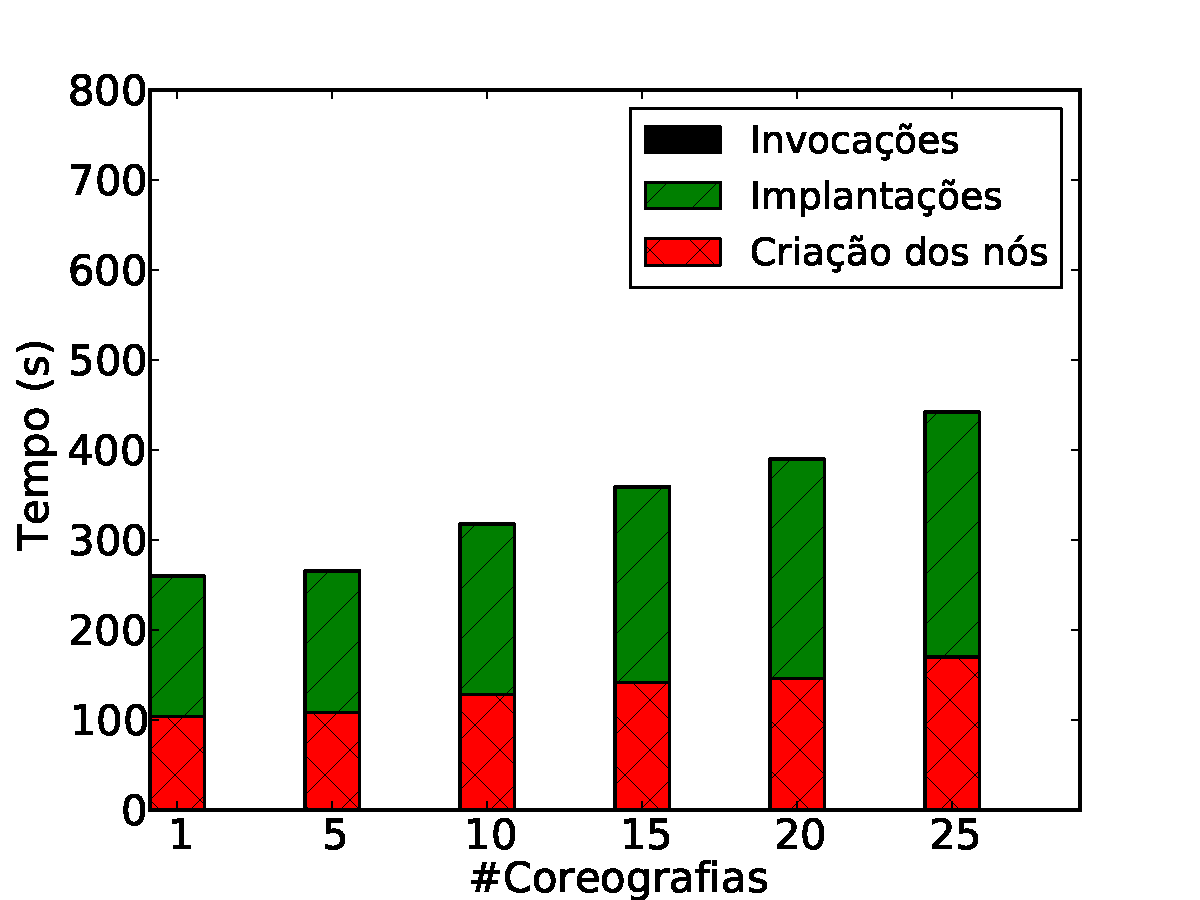
\includegraphics[width=\textwidth]{tempos_medios.pdf}
\caption{Média dos tempos de \\encenação das coreografias}
\label{fig:tempos_medios}
\end{minipage}
\begin{minipage}[b]{0.50\linewidth}
\centering
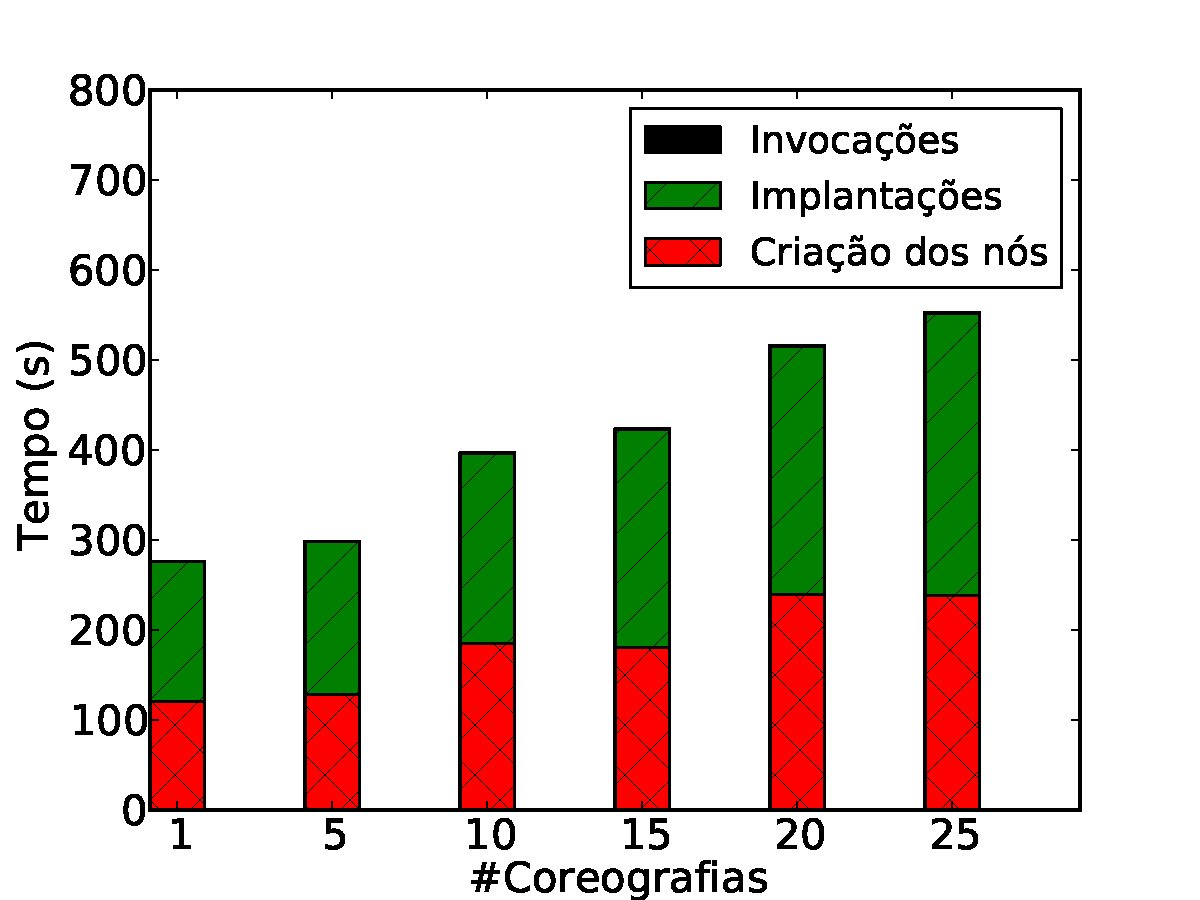
\includegraphics[width=\textwidth]{tempos_totais.pdf}
\caption{Média dos tempos totais de \\encenação das coreografias}
\label{fig:tempos_totais}
\end{minipage}

\end{figure} 

Em nosso experimento observamos que há uma variação no tempo de criação de nós que depende do provedor de IaaS, no nosso caso a Amazon. Esse comportamento consiste na presença de alguns nós que demoram muito mais do que os outros para ficarem prontos. Em alguns casos, o nó requisitado pode não ficar pronto para uso, situação na qual nosso middleware requisita a alocação de um novo nó. A presença desses provisionamentos mais demorados implicam em um aumento considerável nos tempos totais de criação de nós, pois quanto mais nós, maior é a chance da ocorrência de um desses eventos. Em nosso caso, esse aumento foi de 98\% considerando as implantações de 1 e 25 coreografias. No entanto, como se tratam de eventos esporádicos, os tempos médios de criação de nós acabam sendo menos impactado. Em nosso caso, o aumento na média do tempo de criação de nós foi de 64\%

A ocorrência esporádica dos provisionamentos mais demorados de nós explica também o fato de que as medianas para os tempos totais de fases sejam menores do que as médias correspondentes. Portanto, a mediana representa melhor do que a média o valor esperado de um evento como a criação de um nó. Por outro lado, o fato de a mediana dos tempos médios ser bem próxima à média correspondente sugere que os eventos que ``distorcem'' a média dos tempos totais são de fato raros. Outra conclusão que podemos tirar sobre a presença desses eventos esporádicos é a de que não podemos assumir uma distribuição normal para eventos aleatórios de criação de nós. Esses eventos esporádicos também fazem com que os valores representando os desvios dos tempos totais das fases sejam maiores do que os desvios dos tempos médios. 

Outra observação relevante é que os desvios padrões da criação de nós são maiores do que os desvios padrões da implantação de coreografias. Pode-se chegar à mesma conclusão com o coeficiente de variação (razão entre desvio padrão e a média) no lugar do desvio padrão, já que os desvios na criação de nós são maiores do que os desvios das implantações, mesmo sendo os tempos de criação de nós menores do que os tempos de implantação. Essa análise evidencia que a variabilidade do tempo de alocação de um nó pela Amazon é o principal fator na variabilidade do tempo de execução. Em especial, observamos na Tabela~\ref{tab:vm} que os desvios padrões das fases de criação de nós foi muito maior para $N=10$ e $N=20$, o que se deve principalmente aos já mencionados eventos esporádicos. Na Figura~\ref{fig:tempos_totais}, pode-se notar como a presença mais forte dos eventos esporádicos na criação de nós faz com que não haja um crescimento contínuo no tempo total da fase de criação de nós. Outra evidência de como esse comportamento se deve aos eventos esporádicos é a pouca influência no padrão de crescimento dos tempos médios visto na Figura~\ref{fig:tempos_medios}.

O crescimento e a variação observados nos tempos referentes à fase de implantação foram de 75\% para a média do tempo de implantação e 102\%  para a média do tempo da fase de implantação. Esse aumento é de responsabilidade do \ee, e é nosso objetivo diminuir esse aumento o máximo possível. No momento, nossa principal suspeita para o aumento verificado na fase de implantação é a capacidade do Chef Server, uma vez que o servidor em questão manteve-se com 100\% de uso de CPU durante longos períodos, sugerindo que o desempenho pode ser significativamente melhorado através da distribuição e replicação do Chef Server. No entanto, como mencionado, o componente responsável pelo maior impacto negativo na escalabilidade é o serviço da Amazon. É provável que diferentes provedores ofereçam resultados diferentes. Dessa forma, neste trabalho pretendemos ainda realizar a mesma avaliação com pelo menos uma instância do OpenStack. Outra variação na avaliação que pretendemos fazer é aumentar a carga pelo aumento na quantidade de serviços em uma coreografia, em vez de se apenas aumentar a quantidade de coreografias. Embora ambas as variantes aumentem a quantidade de serviços da mesma forma, essa nova variante representa um caso mais típico na implantação de sistemas de grande escala.

